\documentclass[../ECE459FinalProjectReport.tex]{subfiles}

\begin{document}
\chapter{Methodology}
The project simulates the AM and FM communication systems respectively which applies Python 3. The work is done using Jupyter Notebook. Packages imported include \verb|numpy| for numerical computation, \verb|scipy| for signal analysis, and \verb|matplotlib| for plotting.

\section{Choice of Message Signal}

Two message signals are tested in this project:
\begin{enumerate}
    \item The multi-tone sinusoidal signal $m_1 (t) = A_1\cos(2\pi f_1 t + \phi_1) + A_2 \cos(2\pi f_2 t + \phi_2)$.
    \item The TTS-generated male voice recording.
\end{enumerate}

The choice of the multi-tone signal lies in its simplicity as a periodic function and special properties as a linear combination of two sinusoidal functions. Such choice allows the team to observe the distortion by noise in an easier way, as the sinusoidal functions have relatively simple frequency spectrums. The male voice recording enables the team to practice the designed communication system in a more realistic scenario.

Generating the multi-tone signal can be achieved by Python expression
\begin{lstlisting}[language=python]
t = np.arange(0, duration, 1/fs) # time vector
message = A1 * np.cos(2 * np.pi * f1 * t + phi1) + A2 * np.cos(2 * np.pi * f2 * t + phi2)
\end{lstlisting}
and generating the voice signal from a wave audio file can be achieved by
\begin{lstlisting}[language=python]
fs, audio_data = wavfile.read('audio.wav') # fs is the sampling rate of the audio file
t = np.arange(0, len(data)/fs, 1/fs) # time vector
\end{lstlisting}

\section{AM Simulation}
\section{Envelope Modulation}

The modulation of a message signal, denoted as $m(t)$, can be achieved through envelope modulation, represented by the equation:

\begin{equation}
    s(t) = A_c [1 + k_a m(t)] \cos (2\pi f_c t)
\end{equation}

In this expression, $k_a$ denotes the modulation sensitivity, $A_c$ corresponds to the amplitude of the carrier wave, and $f_c$ represents the frequency of the carrier wave. It is imperative to ensure that the carrier wave frequency $f_c$ significantly surpasses the highest frequency component, denoted as $W$, of the message signal $m(t)$ to prevent aliasing. This condition can be expressed as $f_c \gg W$. Moreover, the choice of the modulation sensitivity, $k_a$, needs to adhere to the constraint:

\begin{equation}
    \left| k_a m(t) \right| < 1, \quad \text{for all }t
\end{equation}

This condition is crucial to prevent envelope distortion, as outlined by \textcite[pp. 101-102]{haykinIntroductionAnalogDigital2007}.

The implementation of amplitude modulation (AM) can be illustrated through the block diagram depicted in Figure \ref{fig:env-mod}. For practical implementation in Python, the AM modulation process can be realized using the following code snippet:

\begin{lstlisting}[language=python]
am_signal = Ac*(1 + ka*data) * np.cos(2*np.pi*fc*t)
\end{lstlisting}

Here, \verb|data| refers to the array containing samples of the message signal, and \verb|ka| denotes the modulation sensitivity.

\begin{figure}[b]
    \centering
    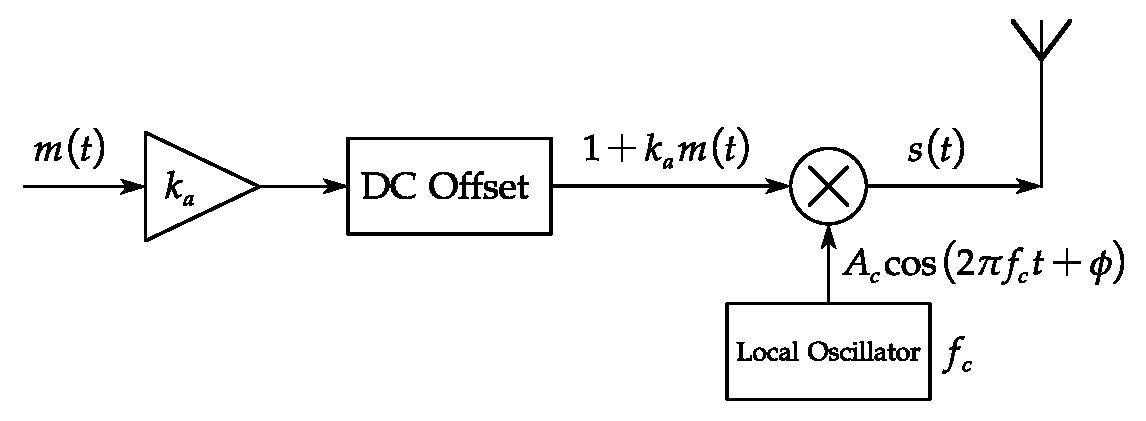
\includegraphics[scale=0.7]{plots/env_mod.pdf}
    \caption{Block diagram illustrating the process of envelope modulation.}
    \label{fig:env-mod}
\end{figure}

\subsection{Envelope Detection}
~
\subsection{SNR Calculation and Measurement}
~
\section{FM Simulation}
\subsection{Narrow-Band FM Modulation}
~
\subsection{Narrow-Band FM Demodulation}
~
\subsection{SNR Calculation and Measurement}
~
\section{Filter Design}
\subsection{Ideal Filters}
% 讲LPF和BPF的TF,然后引出为什么ideal filter无法实现,再引出butterworth
~
\subsection{Butterworth Filter}

Both AM and FM communication systems require filters. Yet in real life, ideal filters are not implementable. However, the Butterworth Filter can behave closely to the ideal filter. According to \cite{storrButterworthFilterDesign2013,kudekiAnalogSignalsSystems2009}, a Butterworth Low Pass Filter has a maximum flat frequency response within its passband and rolls off quickly at the cut-off frequency.

The transfer function of a Butterworth Low Pass Filter is expressed as
\begin{equation}
    \left| H\left( \omega \right) \right|^2=\frac{1}{1+\left( \frac{\omega}{\omega _c} \right) ^{2n}}
\end{equation}
where $n$ is the order of the filter and $\omega_c$ is the cut-off frequency. The higher the order $n$, the closer the Butterworth Filter behaves like an ideal filter. Similarly, the transfer function of a Butterworth Band Pass Filter is???????

According to \textcite{thescipycommunityScipySignalButter,thescipycommunityScipySignalButtera,thescipycommunityScipySignalFiltfilt,thescipycommunityScipySignalLfilter}, the filters can be realized in the following way: ?????????????
%!! Needs Modification!!!!
\begin{lstlisting}[language=python]
# Low Pass Filter
# Get coefficients for butter filter
b, a = signal.butter(4, 100, 'low', analog=True)
w, h = signal.freqs(b, a)
sos = signal.butter(10, 15, 'hp', fs=1000, output='sos')
filtered = signal.sosfilt(sos, sig)

# Band Pass Filter
# Get coefficients for butter filter
b, a = signal.butter(4, [50, 100], 'band', analog=True)
w, h = signal.freqs(b, a)
sos = signal.butter(10, 15, 'hp', fs=1000, output='sos')
filtered = signal.sosfilt(sos, sig)
\end{lstlisting}


\begin{figure}[b]
    \centering
    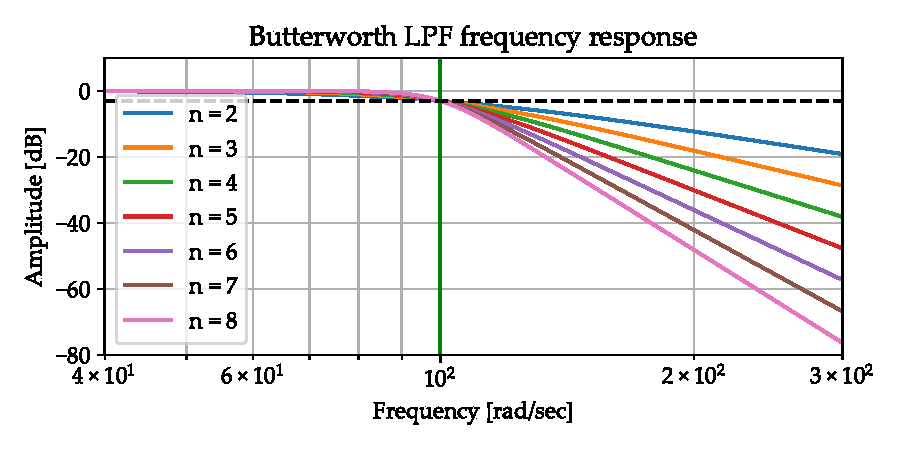
\includegraphics[scale=0.7]{plots/butterworth-lpf.pdf}
    \caption{The frequency response of a Butterworth LPF with cut-off frequency $\omega_c = \SI{100}{\radian\per\s}$. The black dash line shows the \SI{-3}{\dB} amplitude.}
    \label{fig:butter-lpf}
\end{figure}

\begin{figure}[b]
    \centering
    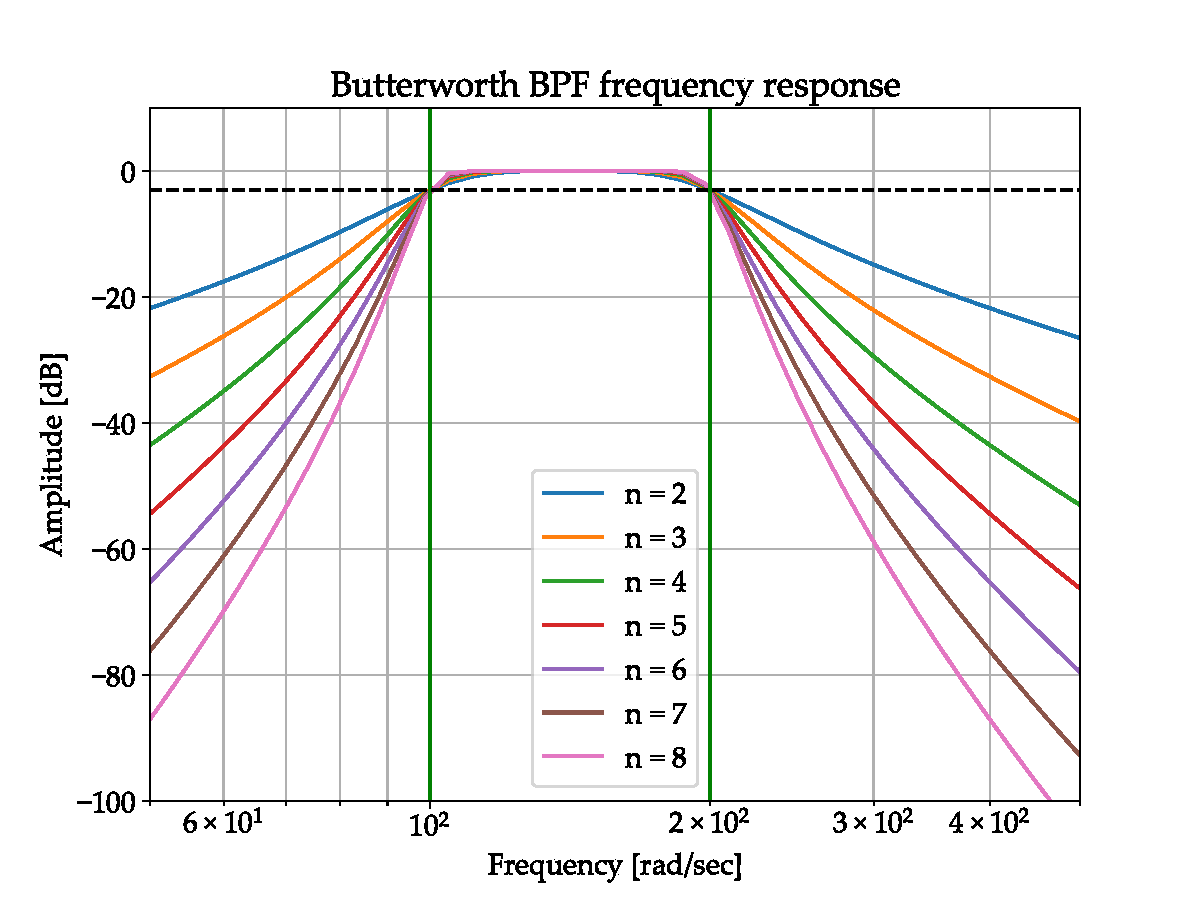
\includegraphics[scale=0.7]{plots/butterworth-bpf.pdf}
    \caption{The frequency response of a Butterworth BPF with cut-off frequency $\omega_c = \SI{100}{\radian\per\s}$. The black dash line shows the \SI{-3}{\dB} amplitude.}
    \label{fig:butter-bpf}
\end{figure}


\section{Additive White Gaussian Noise}
% Definition, principles, and how to generate in Python

\end{document}